\documentclass[fleqn,usenatbib]{mnras}
%=========================================================================
\usepackage{amsmath}
\usepackage{amssymb}
\usepackage{graphicx}
\usepackage{grffile}
\usepackage{float}
\usepackage[dvips]{epsfig}
\usepackage{epsfig}
\usepackage{dblfloatfix}
\usepackage{color}
\usepackage{caption}
\usepackage{hyperref}
\usepackage{bm}
\usepackage[british]{babel}
%Non reposionated tables
\newcommand{\HI}{{\text{H\MakeUppercase{\romannumeral 1}}} }
\newcommand{\lya}{\ifmmode{{\rm Ly}\alpha}\else Ly$\alpha$\ \fi}
\newcommand{\kms}{\ifmmode\mathrm{km\ s}^{-1}\else km s$^{-1}$\fi}
\newcommand{\vrot}{\ifmmode v_{\mathrm{rot}}\else $v_{\mathrm{rot}}$~\fi}
\newcommand{\vout}{\ifmmode v_{\mathrm{out}}\else $v_{\mathrm{out}}$~\fi}
\newcommand{\tauh}{\ifmmode \tau_{\mathrm{H}}\else $\tau_{\mathrm{H}}$~\fi}
\newcommand{\vth}{\ifmmode v_{\mathrm{th}}\else $v_{\mathrm{th}}$~\fi}
\newcommand{\hatk}{\ifmmode \hat{k}\else $\hat{k}$~\fi}
\newcommand{\STD}{\ifmmode \mathrm{STD}\else $\mathrm{STD}$~\fi}
\newcommand{\SKW}{\ifmmode \mathrm{SKW}\else $\mathrm{SKW}$~\fi}
\newcommand{\BI}{\ifmmode \mathrm{BI}\else $\mathrm{BI}$~\fi}

\begin{document}

%=========================================================================
%		FRONT MATTER
%=========================================================================
\title[The Local Group in Simulations]{Finding the Local Group in 
cosmological hydrodynamical simulations}  

\author[Catalina G\'omez et al.]{
  Catalina G\'omez$^{1}$
  \thanks{c.gomez10@uniandes.edu.co},
  Jaime E. Forero-Romero $^{2}$
  \&
  More Friends $^{3}$
  \\
  %%
  $^{1}$ Departamento de Ingenier\'ia Biom\'edica, Universidad de los
  Andes, Cra. 1 No. 18A-12, CP 111711, Bogot\'a, Colombia \\
  $^{2}$ Departamento de F\'isica, Universidad de los Andes, Cra. 1
  No. 18A-10 Edificio Ip, CP 111711, Bogot\'a, Colombia \\
  $^{3}$ Somewhere Over the Rainbow\\
}

\maketitle

\begin{abstract}

 \end{abstract}


\section{Introduction}
 
\section{Related Work}
Previous studies have found a range of estimates of the individual
masses of the MW and M31, or the total mass of the LG
\citep{2016MNRAS.457..844F}, limiting the straightforward/direct
comparison between simulations and the observed Local Group. The
selection of viable Local Group candidates from simulations relies on
the kinematics of the LG members, but the density of systems that
fully resemble the LG is low. Below there is a review of the
literature, and the values of selection criteria used in different
scenarios.   

%We are not the 99 percent: quantifying asphericity in the distribution of Local Group satellites: https://arxiv.org/pdf/1805.03188.pdf
Recently \cite{2018MNRAS.478.5533F} proposed a characterization of the
global satellite distribution ranked by different selection
criteria. The samples were generated from three simulations:
Illustris-1, Illustris-1-Dark and ELVIS. The procedure they used to
select the halo pairs that resemble the LG is described below. The
mass constraint is applied to halos with a stellar mass within the
range $[1\times 10^{10} M_\odot, 1\times 10^{11} M_\odot]$. Then, the
pair candidates (A,B) were selected by searching for mutually closest
halos, but restricted with the separation distance between them to be
at least $700$ $kpc$. An isolation criterion was defined to keep the
pairs in which there are no other galaxies with a mass greater than
the minimum mass of the pair within a distance of $3d_{A,B}$. Finally,
the relative radial velocity was restricted to be in the range $-120
kms^{-1}<V_r<0 km s^{-1}$.  


%APOSTLE: https://arxiv.org/pdf/1507.03643.pdf
Based on the match with kinematics of the LG members, \cite{fattahi2016apostle} found the constraints on the mass of the LG and compared it with estimates from other methods. The candidates were selected from the Millennium Simulations (I and II) and used for resimulations at different resolution levels. The reference conditions for the MW-M31 pair were defined as follows: the separation distance between the two galaxies is $787 \pm 25$ $kpc$, the approaching velocity (relative radial velocity) is $123 \pm 4$ $kms^{-1}$, the tangential velocity is $7$ $kms^{-1}$. Additionally, there is an isolation environment around \cite{forero2018we}
the pair: there are no galaxies brighter than the Large Magellanic Cloud within 3 Mpc from the MW. 

The first constraint is applied on the separation distance between the pair members, keeping the ones separated by a distance within the range $[600kpc-1.0Mpc]$. Next, the virial mass of each pair member (that fulfill the previous constraint) must not exceed $10^{11} M_\odot$, and the pair mass must be less than $10^{13} M_\odot$. These pairs must be in an isolated medium, which means that the cannot be other halo more massive than the less massive member of the pair within $2.5Mpc$ from the center of the pair. They evaluated different values for this threshold distance, making the isolation more or less restricted. To visualize the total mass distribution of the pairs that satisfy the previous conditions, they included three new criteria that can be imposed individually or combined. These are the following: (i) the relative radial velocity is within the range $[-175,75]$ $kms^{-1}$; (ii) the tangential velocity within the range $[0,50]$ $kms^{-1}$, and (iii) the Hubble flow velocity is in the observed range. Only 14 pairs satisfied the velocity criteria simultaneously. Furthermore, from these 14 pairs, the authors selected a subsample for the resimulation using more flexible constraints, and analyzed the the properties (brightness, mass, velocities) of the satellite population around each pair.

An important finding from the selection procedure proposed by \cite{fattahi2016apostle} was that the relative radial velocity constraint favors high-mass pairs $(5\times 10^{12} M_\odot)$, while the tangential velocity constraint low-mass pairs $(6\times 10^{11} M_\odot)$

%The mass distribution and gravitational potential of the MW:https://arxiv.org/pdf/1608.00971.pdf

%THE KINEMATICS OF THE LOCAL GROUP IN A COSMOLOGICAL CONTEXT: https://arxiv.org/pdf/1303.2690.pdf
%important figures: #1 


%THE LOCAL GROUP IN THE COSMIC WEB: https://arxiv.org/pdf/1408.3166.pdf
%important figures: #1, #4

%The dark matter assembly of the Local Group in constrained cosmological simulations of a ΛCDM universe: https://arxiv.org/pdf/1107.0017.pdf
%important figures: #2

%THE STELLAR MASS STRUCTURE OF MASSIVE GALAXIES FROM Z = 0 TO Z = 2.5; SURFACE DENSITY PROFILES AND HALF-MASS RADII: https://arxiv.org/pdf/1208.4363.pdf
\section{Methods}
\textit{Simulation datasets}\\
In this work we used the simulations from the TNG project.


\textit{Catalogue Selection}\\
We defined two strategies to create samples of galaxies by imposing an initial cut on Dark Matter Halo Mass and Stellar Mass. %como definimos DM halo mass? decir que solo tomamos informacion de los subgrupos/subhalos
Then, we find candidate pairs applied more constraints on other properties including the relative separation, an isolation medium and the relative velocities. A pair is considered when two galaxies are closer to each other. To search for pair candidates, padding was applied in all the dimensions of the simulation box by replicating it. The values constraints are described below:
\begin{enumerate}[i]
  \item Pair candidates with a stellar mass in the range $10^{10}M_\odot <M_\star<1.5\times 10^{10}M_\odot$.Pair candidates with a dark matter halo mass in the range $10^{11}M_\odot<M_{halo}<10^{12}M_\odot$. Additionally, the corresponding subhalo must be central, and its stellar mass must be different from zero. 
  \item The relative separation between the pair ($d_{AB}$)must be at least $700$ kpc. 
  \item Keep the isolated pairs by discarding the ones with any other galaxy within a radius of $3\times d_{AB}$, with a mass greater than the minimum mass of the pair. 
  \item The relative radial velocity between the two galaxies of the pair must be in the range $-120 km s^{-1}<V_r<0 km s^{-1}$. 
\end{enumerate}
%en DM selection se agrego que sea central y stellar mass diferente de cero

%hablar de combined sample
We present a new perspective in which criteria is defined following the observational values reported for the properties of the Local Group. These values have a degree of uncertainty, which we fixed to make the constraints broader. The values are presented in table \ref{tab:constraints} with the other ranges defined to create the samples based on the Dark Matter halo and stellar mass. To define the new perspective, we applied both individual and combined mass constraints. 
%agregar si se aplico restriccion de centrales o no
\begin{table*} 
\begin{center}
\caption{Summary of the constraint values used to select each sample.}
\label{tab:constraints}
%\resizebox{\columnwidth}{!}{ %Comando para ajustar a columna
\begin{tabular}{|c| c | c | c | c | c |}
\hline
%\multicolumn{6}{|c|}{\textbf{3FCV}} \\ \hline
Step &Property & Stellar & DM &Observations & Broader\\ \hline
1&Stellar mass [$M_\odot$] &[$10^{10}$,$1.5\times 10^{11}$] & $\neq 0$& [$10^{10}$,$10^{11}$]& [$10^{10}$,$10^{11}$]\\

1& Dark matter halo mass [$M_\odot$]& -& [$10^{11}$,$10^{12}$]&[$10^{11}$,$10^{13}$]&[$10^{11}$,$10^{13}$] \\

1 & Stellar mass of the pair [$M_\odot$] &- & -& [$1.29\times10^{11}$,$1.97\times10^{11}$ ]& [$4.89\times10^{10}$,$2.77\times 10^{11}$]\\

1 & DM mass of the pair [$M_\odot$]& -& -&[$2.1\times 10^{12}$, $5.7\times 10^{12}$] & [$$,$9.90\times10^{12}$]\\

2& Relative distance  [kpc]&$\geq700$ &$\geq 700$& [712,862] &[537,1037] \\

3& Isolation radius [kpc]& $3\times d_{AB}$&$3\times d_{AB}$& 1900& 500\\

4& Radial Velocity [km/s]&[-120,0] & [-120,0]& [-135,-111]& [-163,-83]\\
5 & Tangential Velocity [km/s]& -& -& $\leq 66$& $\leq220$\\


\end{tabular}
\end{center}
\end{table*}

Furthermore, we explore other properties for the pairs at each step. The formation time, defined as the redshift or snapshot number when the galaxy had half of its mass, and the last major merger time.

\section{Results}
The change in the number of pairs at each selection step is shown in figure \ref{fig:pairs}, and also, as a density function defined with the respective volume of each simulation. There is a clear tendency of a decreasing number of pairs as progressing from the first criterion to the last one. Even though the number of pairs in Illustris-100 is less than in Illustris-300, when the density is compared, there is almost no change among simulations at different resolutions. The isolation criterion (from step 2 to 3) decreases the number of pairs in a stronger way for the stellar and dark matter samples. However, in the third sample, the number of pairs is decreases more when applying the threshold distance criterion (from step 1 to 2), given that the isolation criterion only restricts $500 kpc$ around the pair.

When comparing the number of pairs among the three different samples (stellar, DM and combined), there are more pairs at each step when the first cut is on the dark matter halo mass. This could be attributed to the number of objects that lie in the range of the mass constraint, which leads to a larger number of pairs at the end of the selection process. 

%ya se sabe que las propiedades del LC son atipicas, lo verificamos con la muestra creada con valores observacionales
Using Illustris-300 at the largest resolution, the sample defined with the observational constraints had almost no pairs left after the preliminary mass constraint. Only one pair fulfilled the combined mass criterion, but not the consecutive ones. As expected, these constraints are rare and even with a large simulation box there are no samples at these ranges. A larger simulation box should be required to observe the rare examples that most fully resemble the Local Group members. 

To avoid loosing galaxies when using the observational constraints, we made the ranges broader and analyzed the properties of the remaining pairs at each step. The final ranges for this sample are shown in the last column of table \ref{tab:constraints}.

%mas parecido entre TNG-100 y TNG-300 con mas particulas
\begin{figure}
\centering
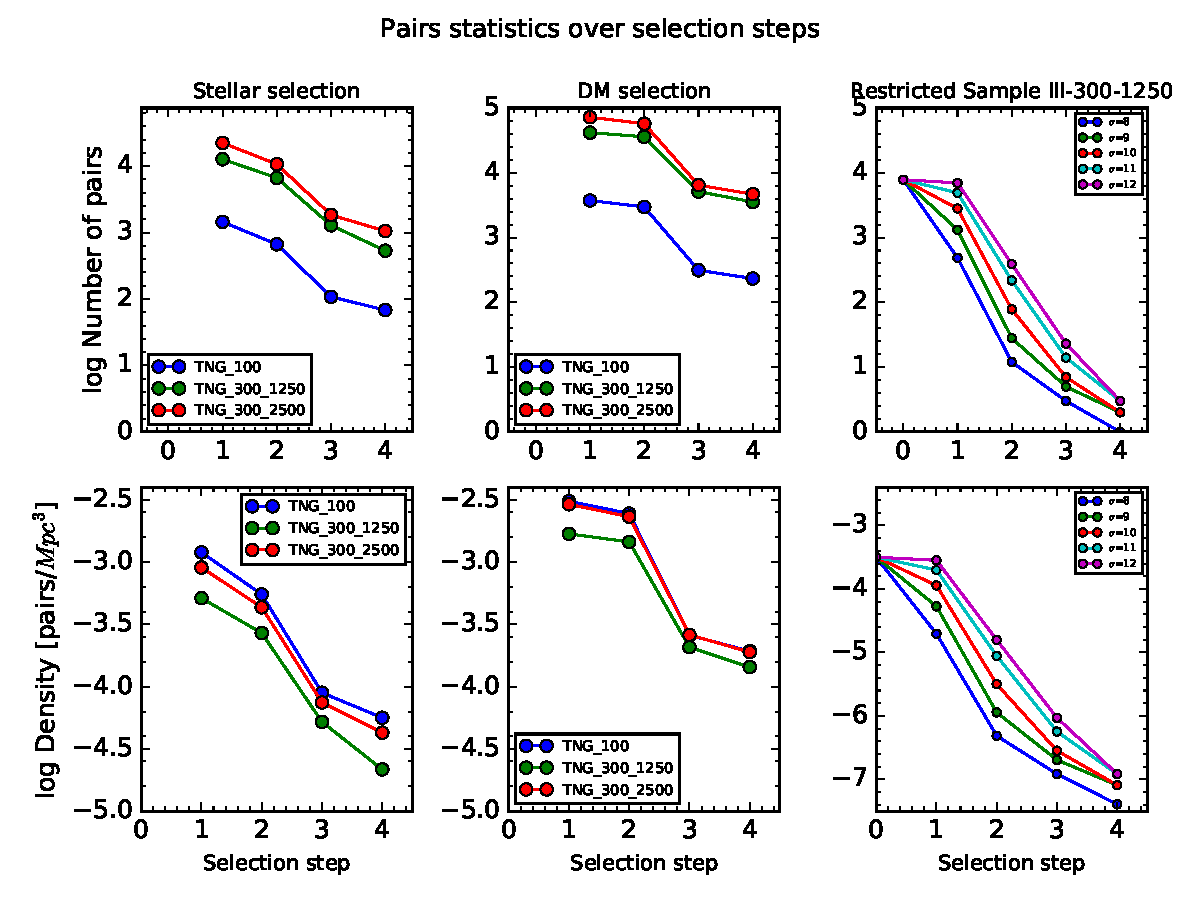
\includegraphics[scale=0.43]{NumberPairs.pdf}
\caption{\label{fig:pairs} Count of pairs (top row) and density defined as $[pairs/Mpc^3]$ at each selection step. In the left and center columns, stage \textit{0} corresponds to the original sample (no pairs defined), and in the right column to the preliminary mass cut.}
\end{figure}
 
 
We calculated the average properties of the pair samples for the different perspectives at each step and compare them between different simulations. The numbers in the x-axis correspond to the four constraints. The properties that are relative to a pair are reported after pair candidates have been selected, which means after applying the mass cut at step 1. 
%comentarios graficas 
When the sample is initially constrained in the stellar mass of the subhalo, the corresponding dark matter halo mass is large. 
 
\begin{figure*}
\centering
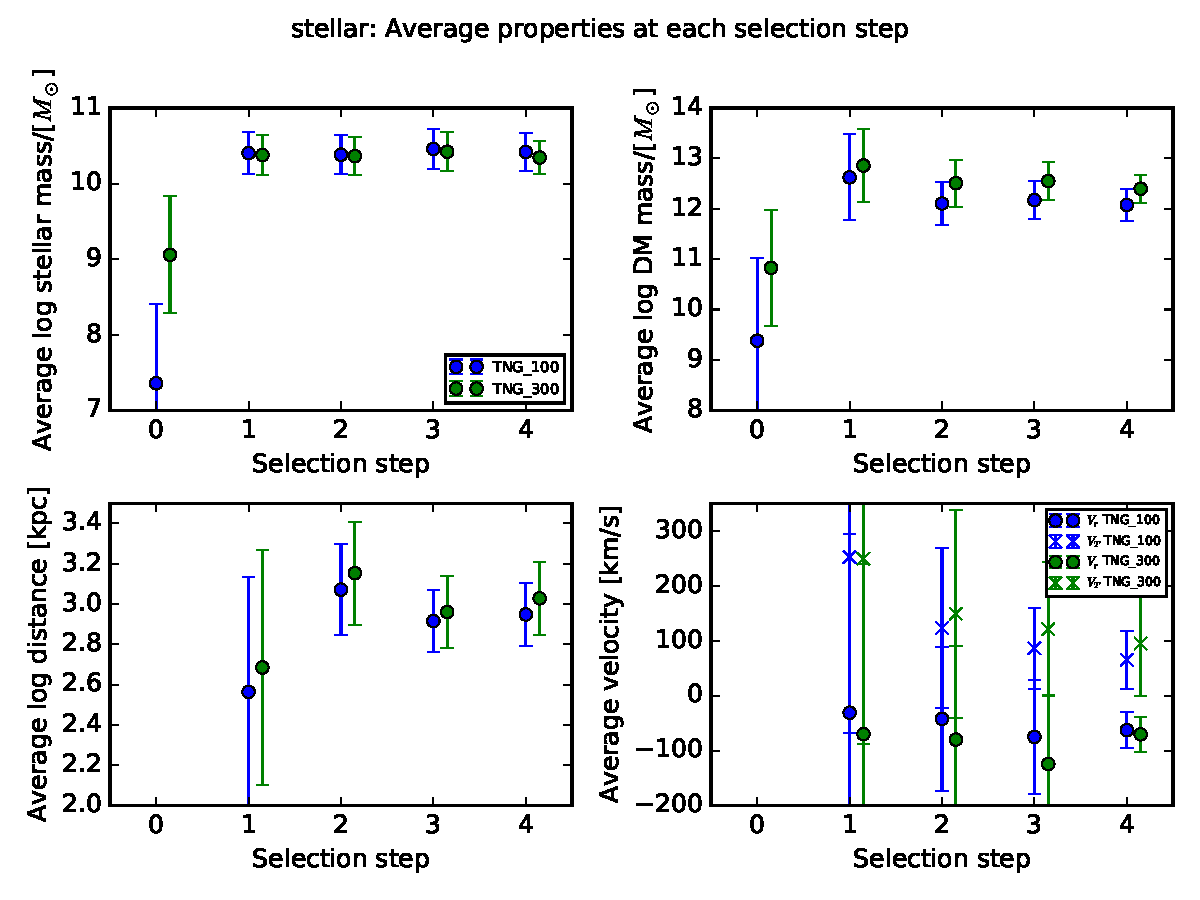
\includegraphics[scale=0.4]{avgProp/stellar_avgPropsTNG_100TNG_300.pdf}
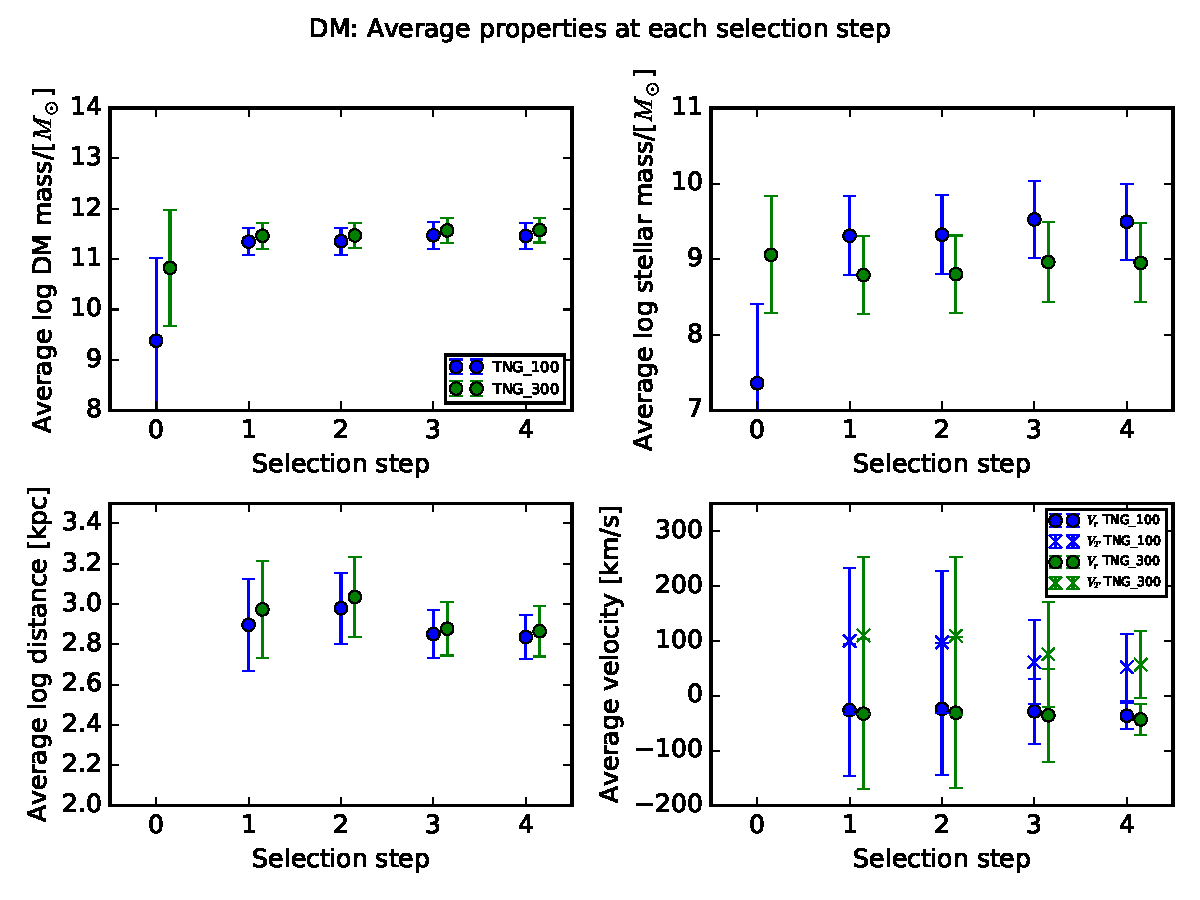
\includegraphics[scale=0.4]{avgProp/DM_avgPropsTNG_100TNG_300.pdf}
\caption{\label{fig:prop_100_300} Comparison between the average properties at each selection step for Illustris-100 and Illustris-300 (1820 and 1250 particles, respectively). Stage $0$ denotes the original sample.}
\end{figure*}

\begin{figure*}
\centering
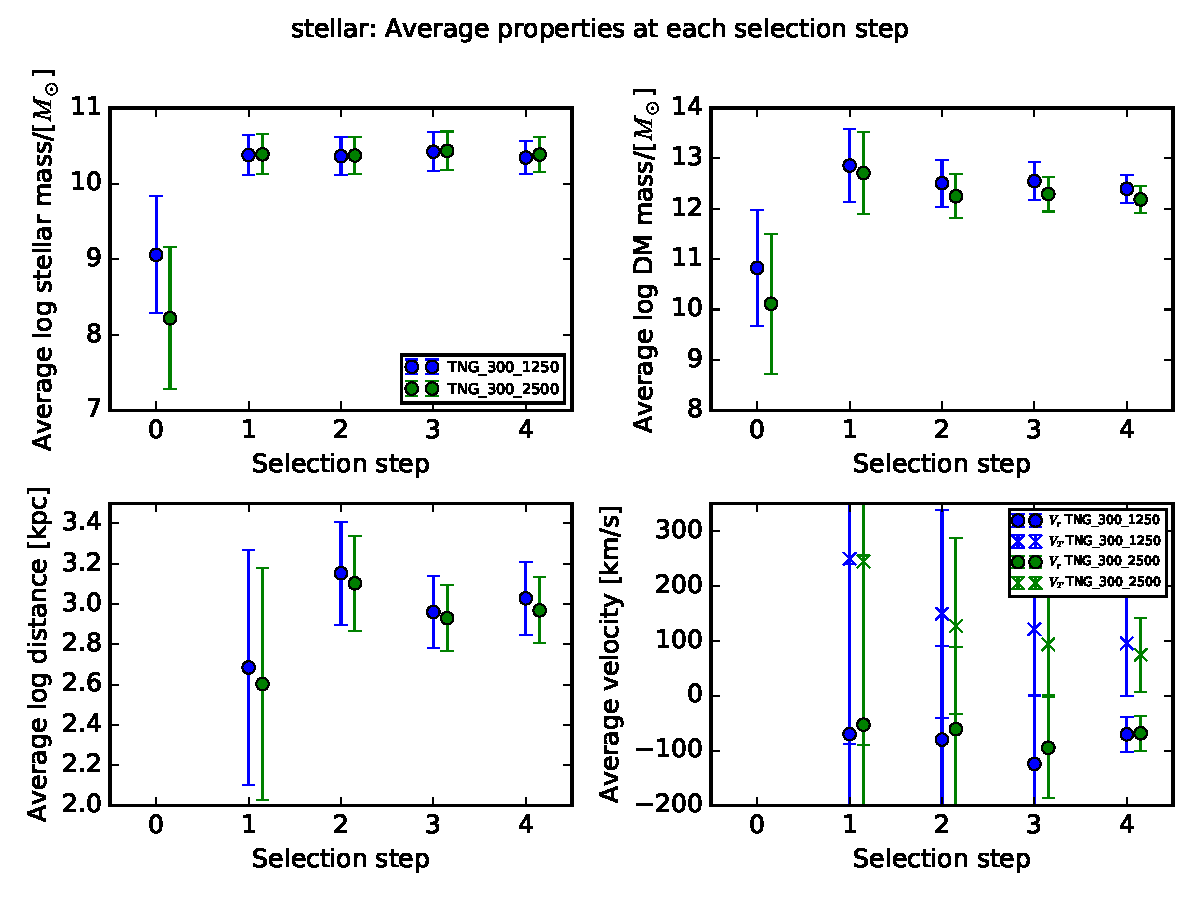
\includegraphics[scale=0.4]{avgProp/stellar_avgPropsTNG_300_1250TNG_300_2500}
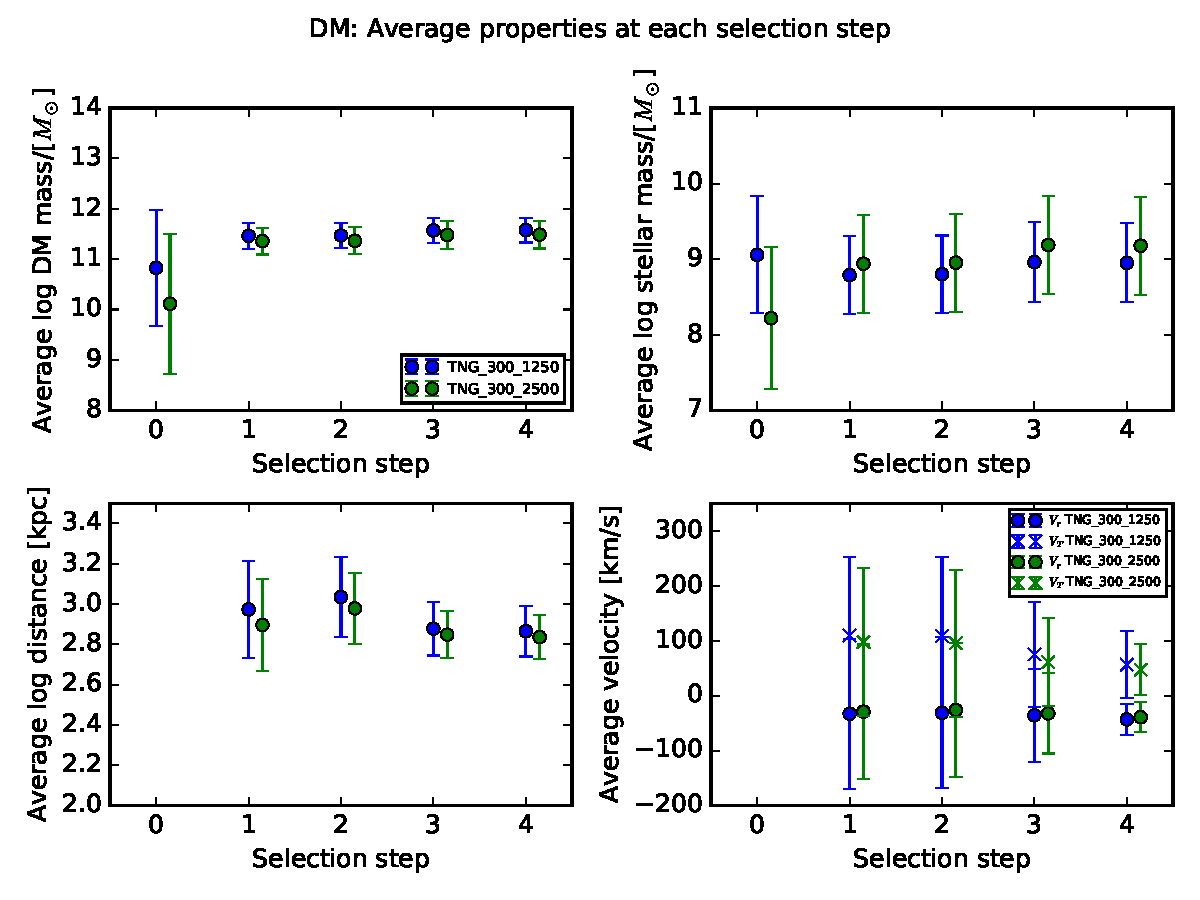
\includegraphics[scale=0.4]{avgProp/DM_avgPropsTNG_300_1250TNG_300_2500}
\caption{\label{fig:prop_300_300} .Comparison between the average properties over each selection step for Illustris-300 at two different resolutions (1250-2500 particles). Stage $0$ denotes the original sample.}
\end{figure*}

%comparacion de propiedades a traves de diferentes muestras para una resolucion fija 
In figure \ref{fig:prop_persp} we compare the average properties of the pairs at each selection step for the three different samples. In the sample constructed from the broader observational values, the mass cut (step 1) includes the preliminary range and the constraint on the mass of the pair, and the velocity cut restricts both the radial and tangential velocities. 
\begin{figure}
\centering
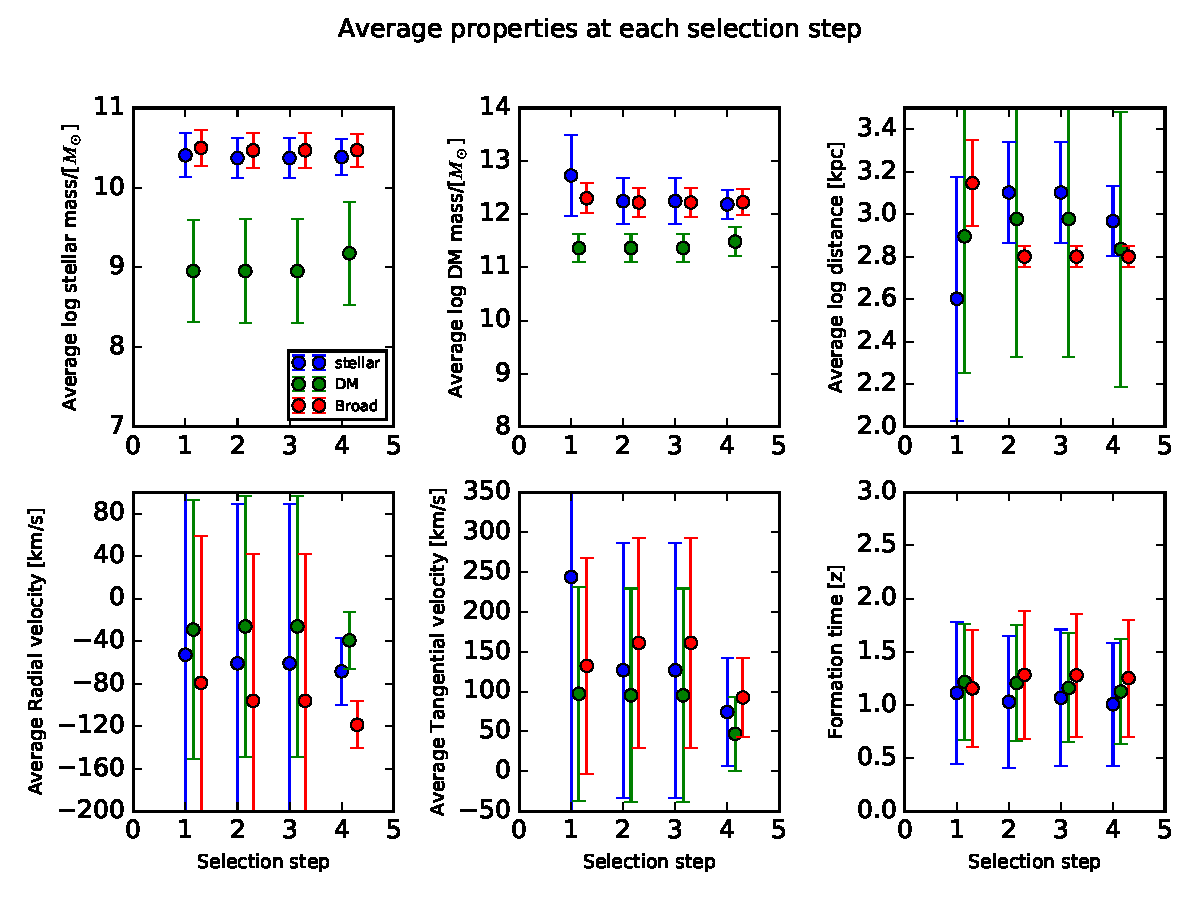
\includegraphics[scale=0.5]{avgProp/ALLavgProps_205_2500.pdf}
\caption{\label{fig:prop_persp} Comparison between the average properties at each selection step for the three perspectives in the simulation Illustris TNG-300-2500.}
\end{figure}


%2D histograms
In figures \ref{fig:2d_vels_ratios} and \ref{fig:2d_times} we visualize the distributions of velocities, stellar and dark matter halo mass ratios of the pair, defined as the minimum over maximum mass, and the times related to the subhalos history. The color represents the count at each bin. 
\begin{figure*}
\centering
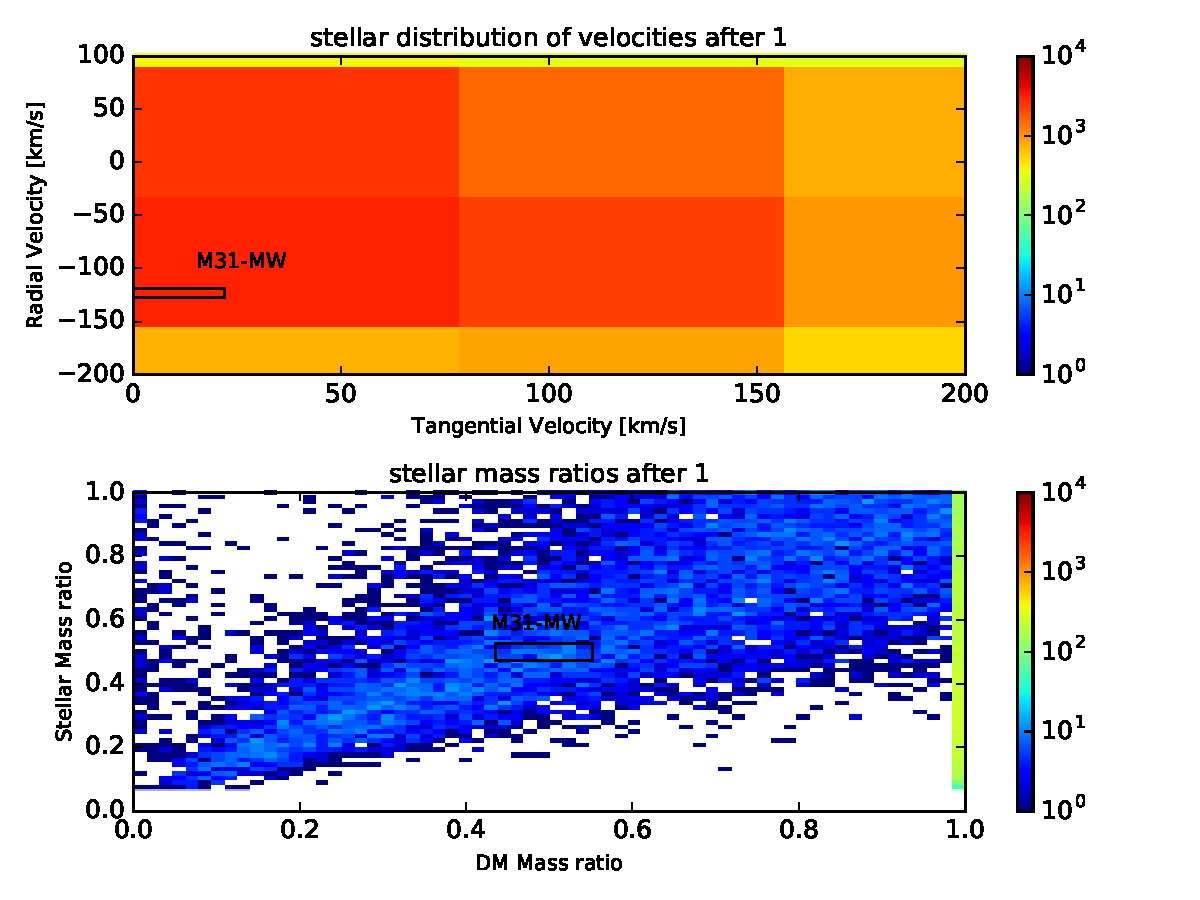
\includegraphics[scale=0.27]{avgProp/stellar_2Dhists_1.pdf}
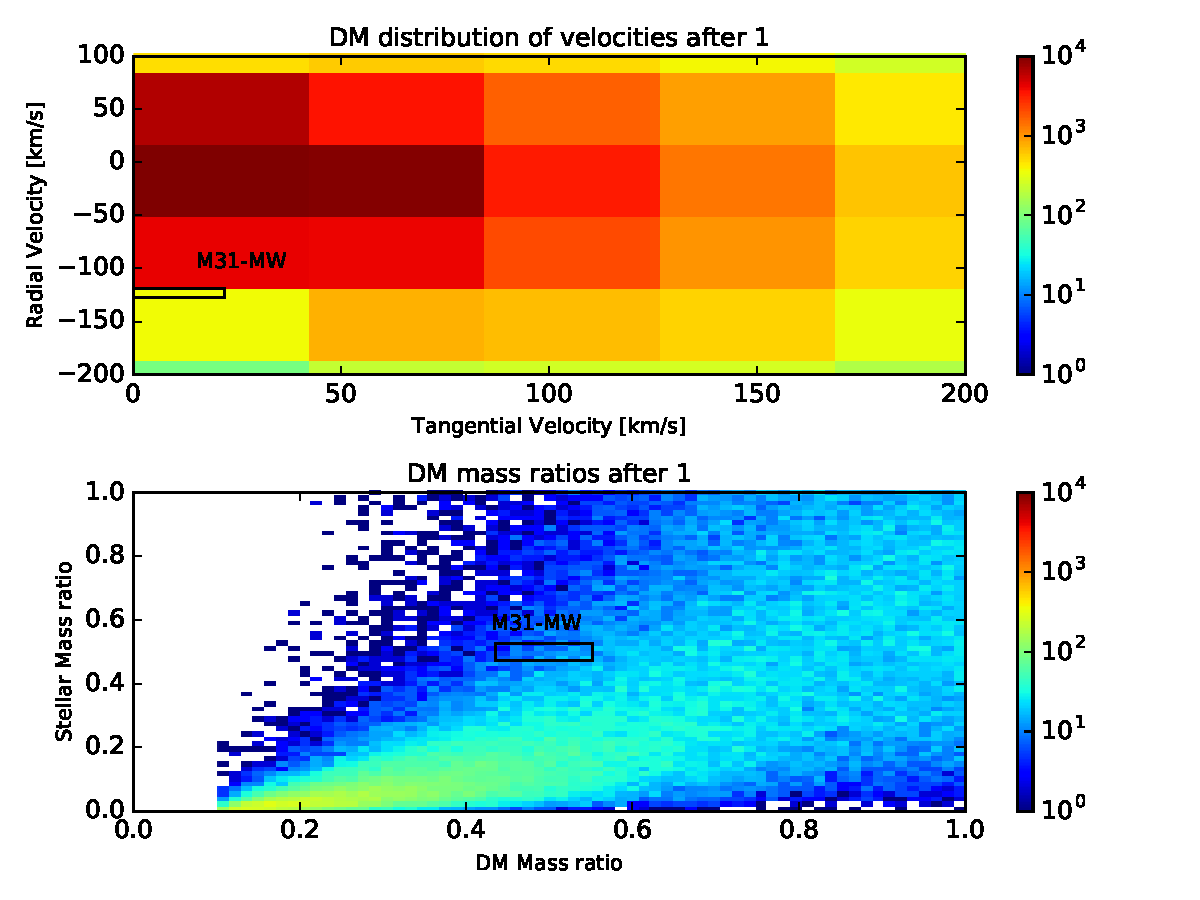
\includegraphics[scale=0.27]{avgProp/DM_2Dhists_1.pdf}
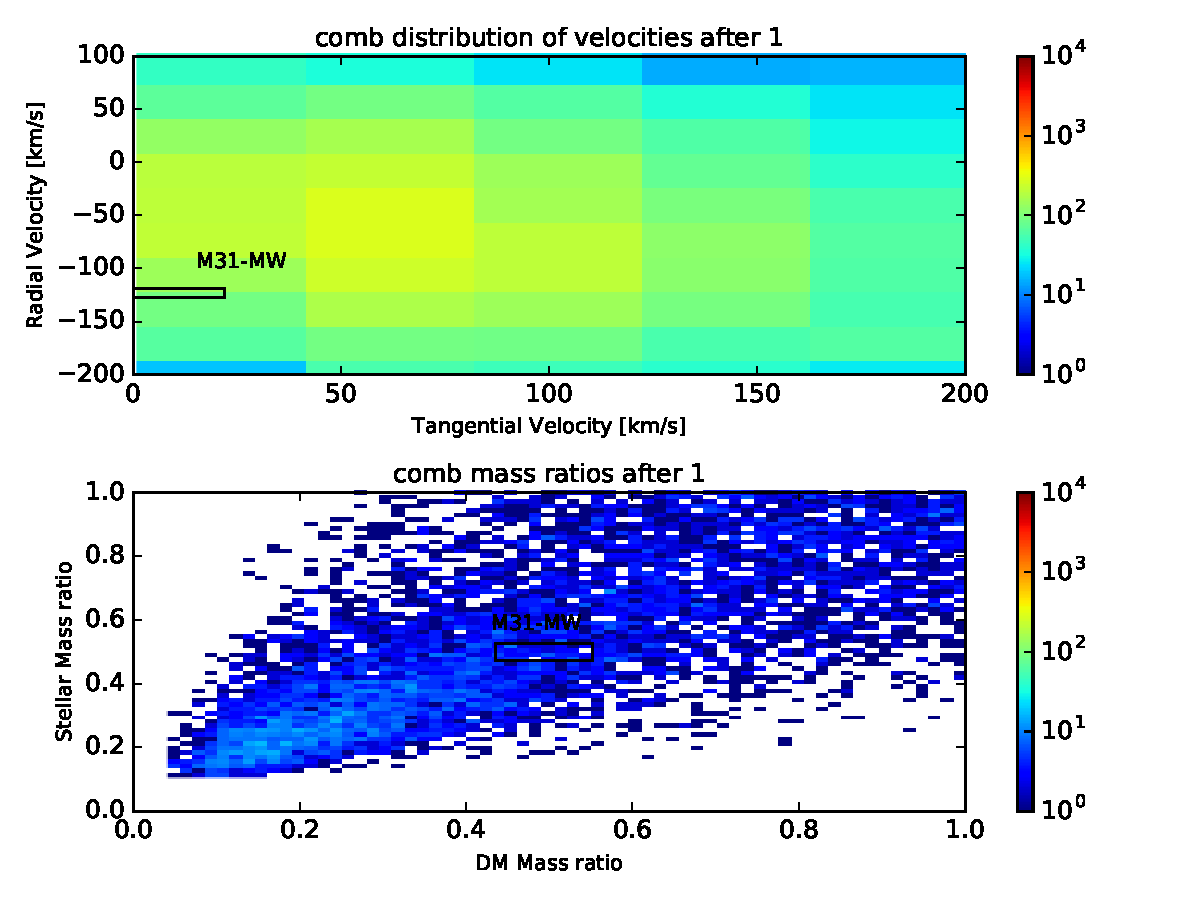
\includegraphics[scale=0.27]{avgProp/comb_2Dhists_1.pdf}
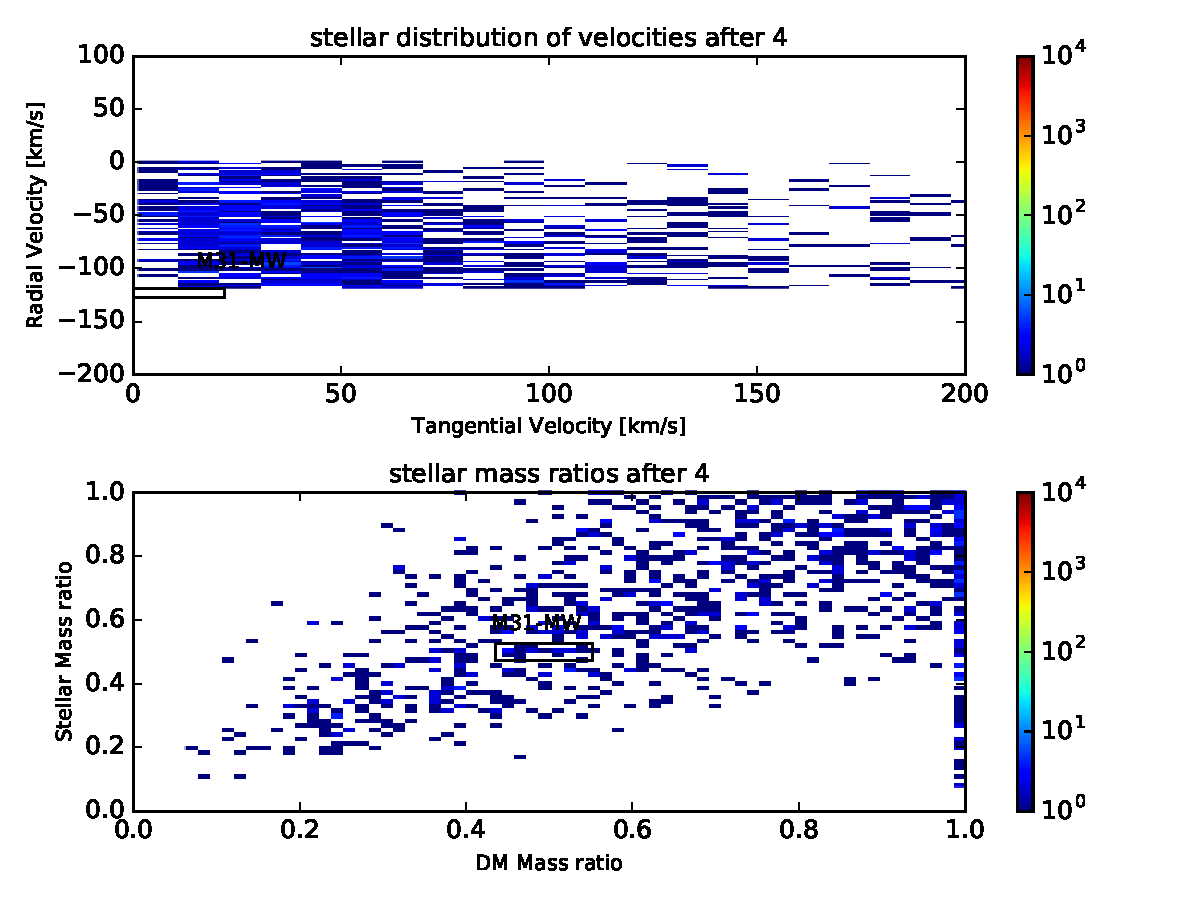
\includegraphics[scale=0.27]{avgProp/stellar_2Dhists_4.pdf}
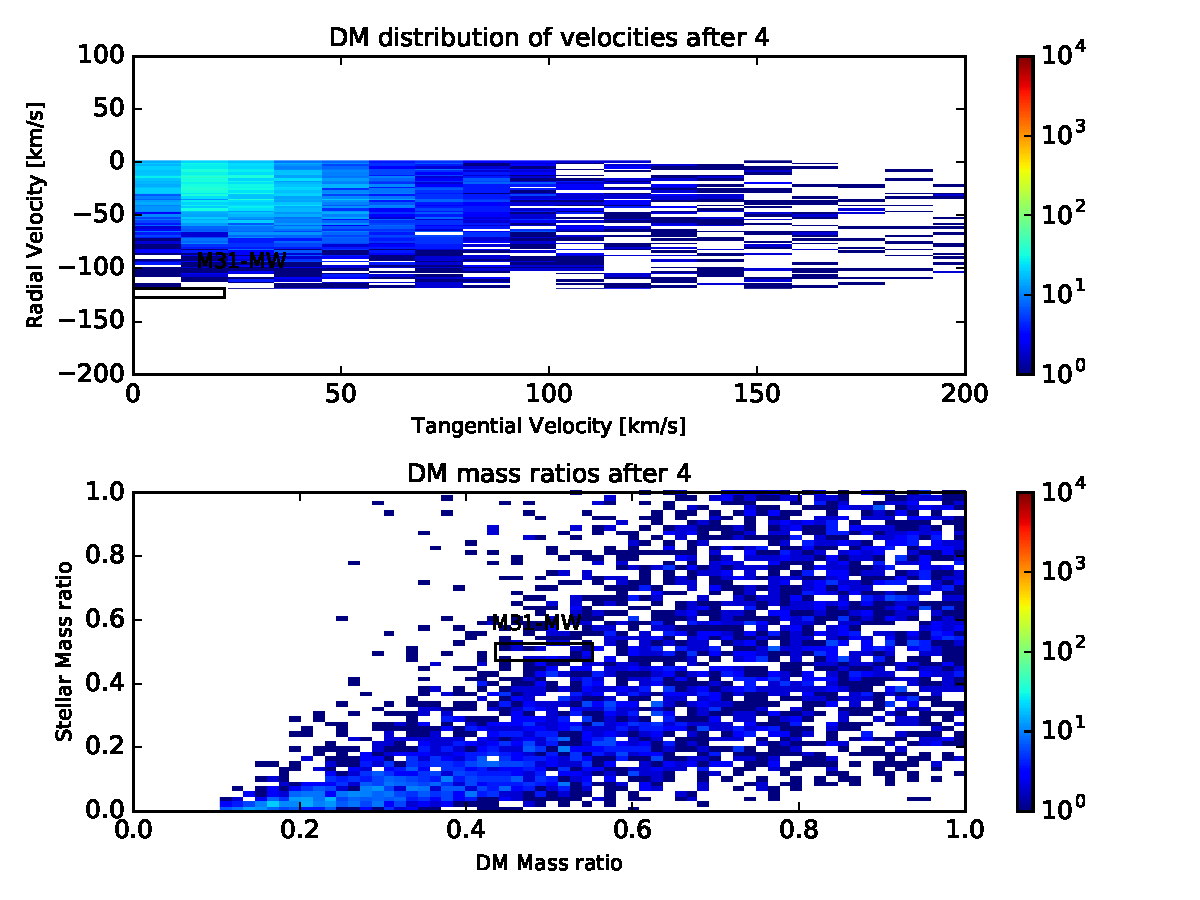
\includegraphics[scale=0.27]{avgProp/DM_2Dhists_4.pdf}
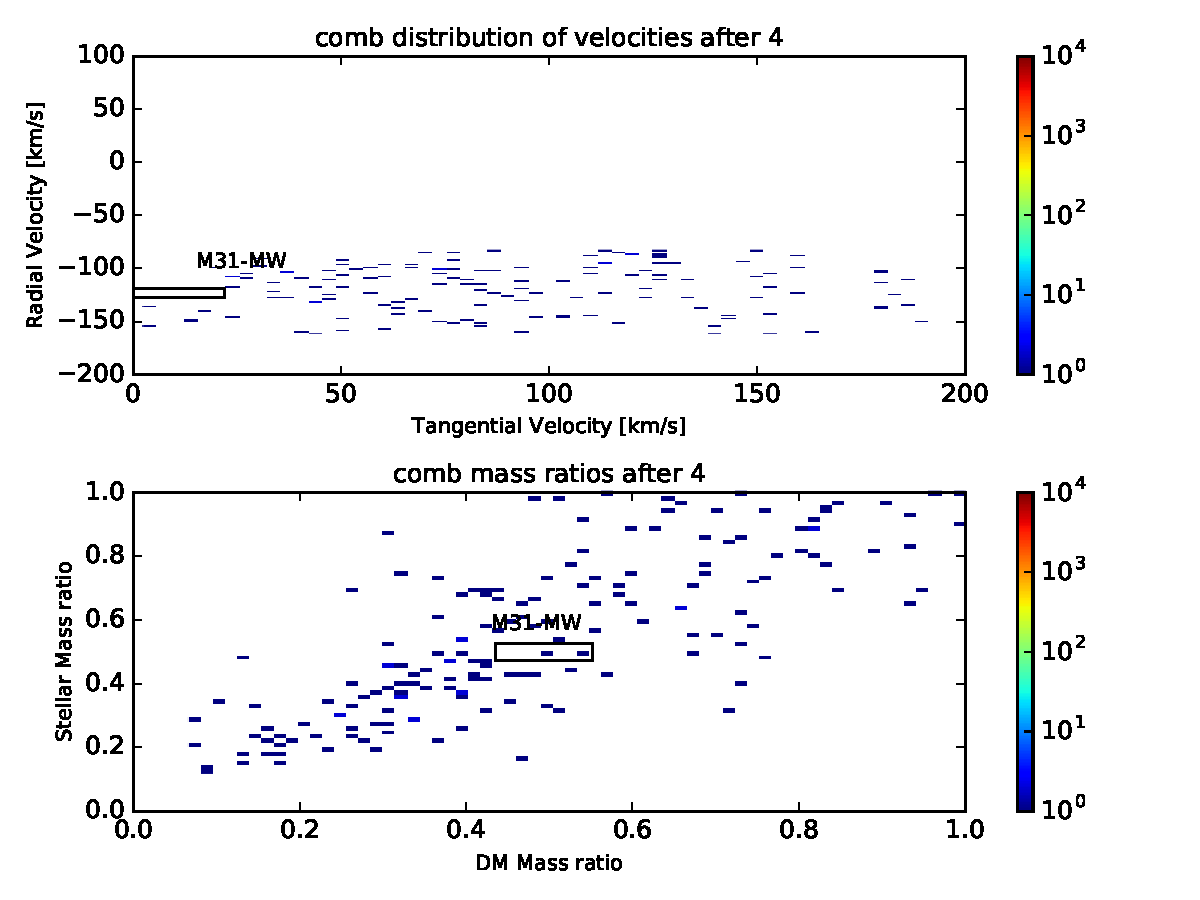
\includegraphics[scale=0.27]{avgProp/comb_2Dhists_4.pdf}
\caption{\label{fig:2d_vels_ratios} 2D histograms of radial and tangential velocities, and stellar and dark matter ratios. From left to right: stellar mass, dark matter halo mass and broader observational values. Top row: distribution after applying the mass cut, bottom row: distribution after the velocity cut.}
\end{figure*}

\begin{figure*}
\centering
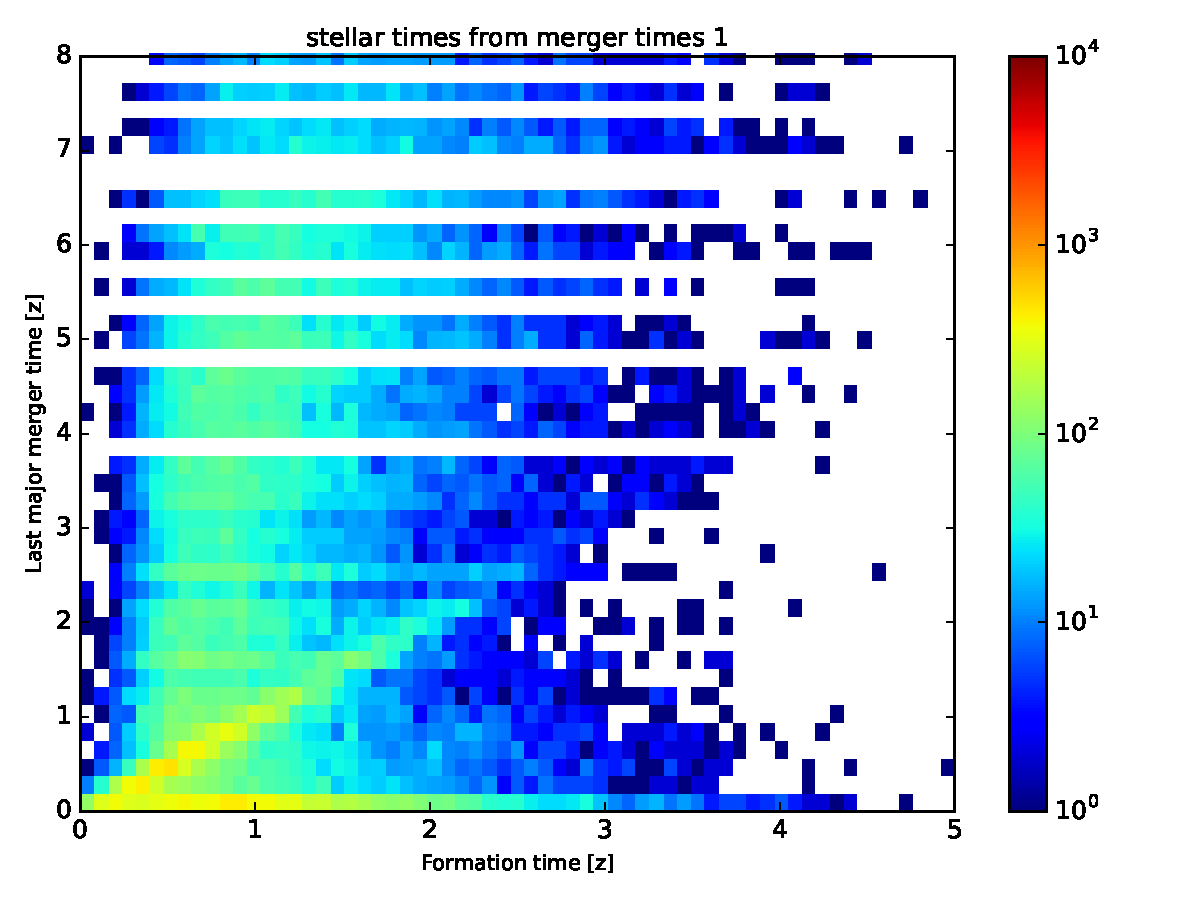
\includegraphics[scale=0.27]{avgProp/stellar_2DhistTimes_1.pdf}
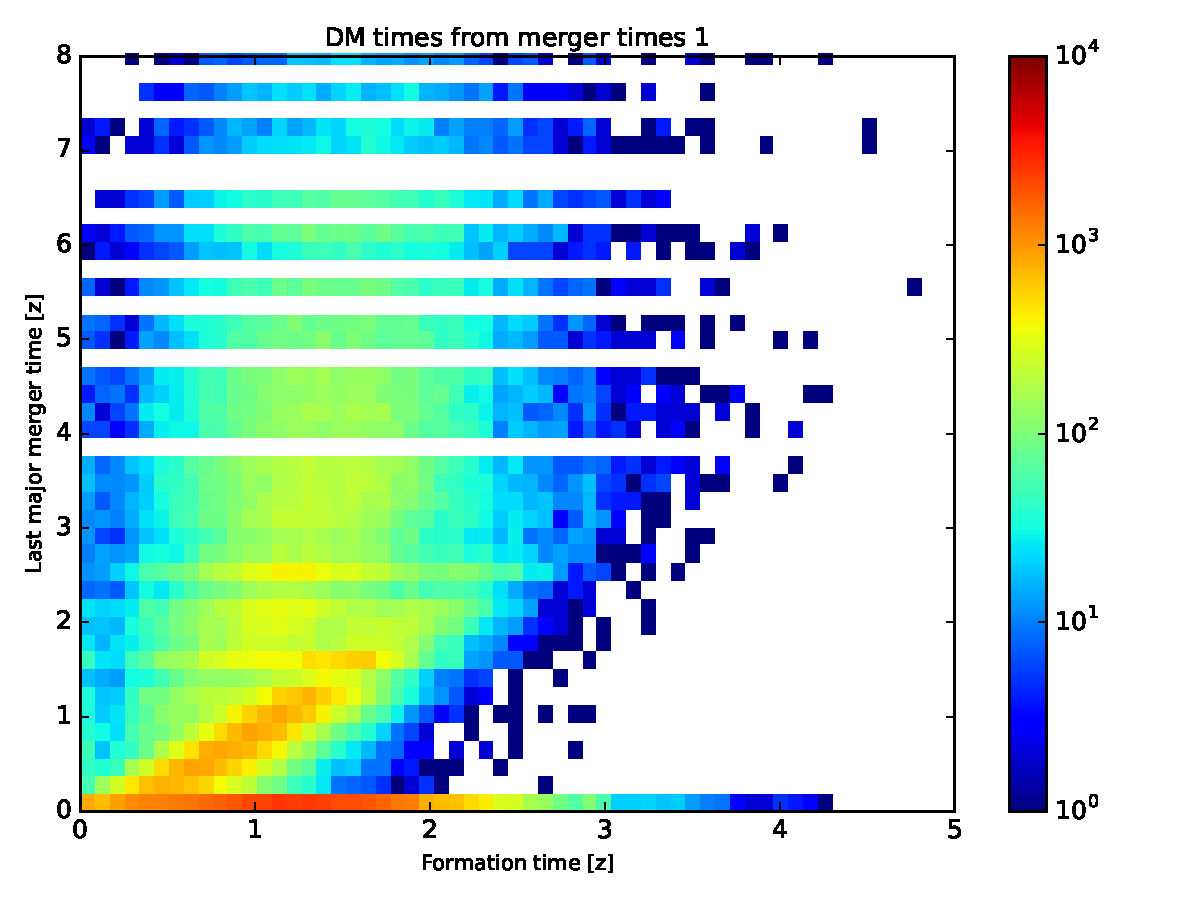
\includegraphics[scale=0.27]{avgProp/DM_2DhistTimes_1.pdf}
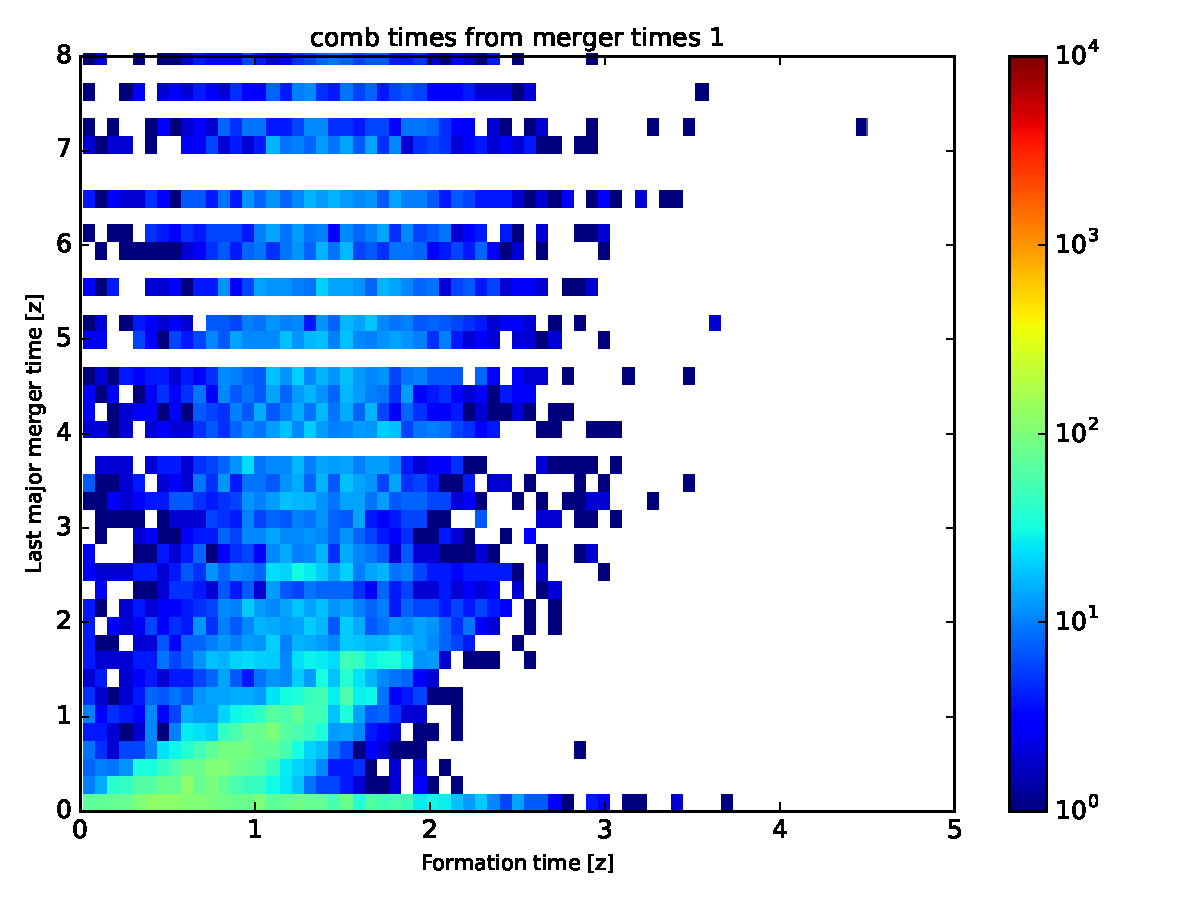
\includegraphics[scale=0.27]{avgProp/comb_2DhistTimes_1.pdf}
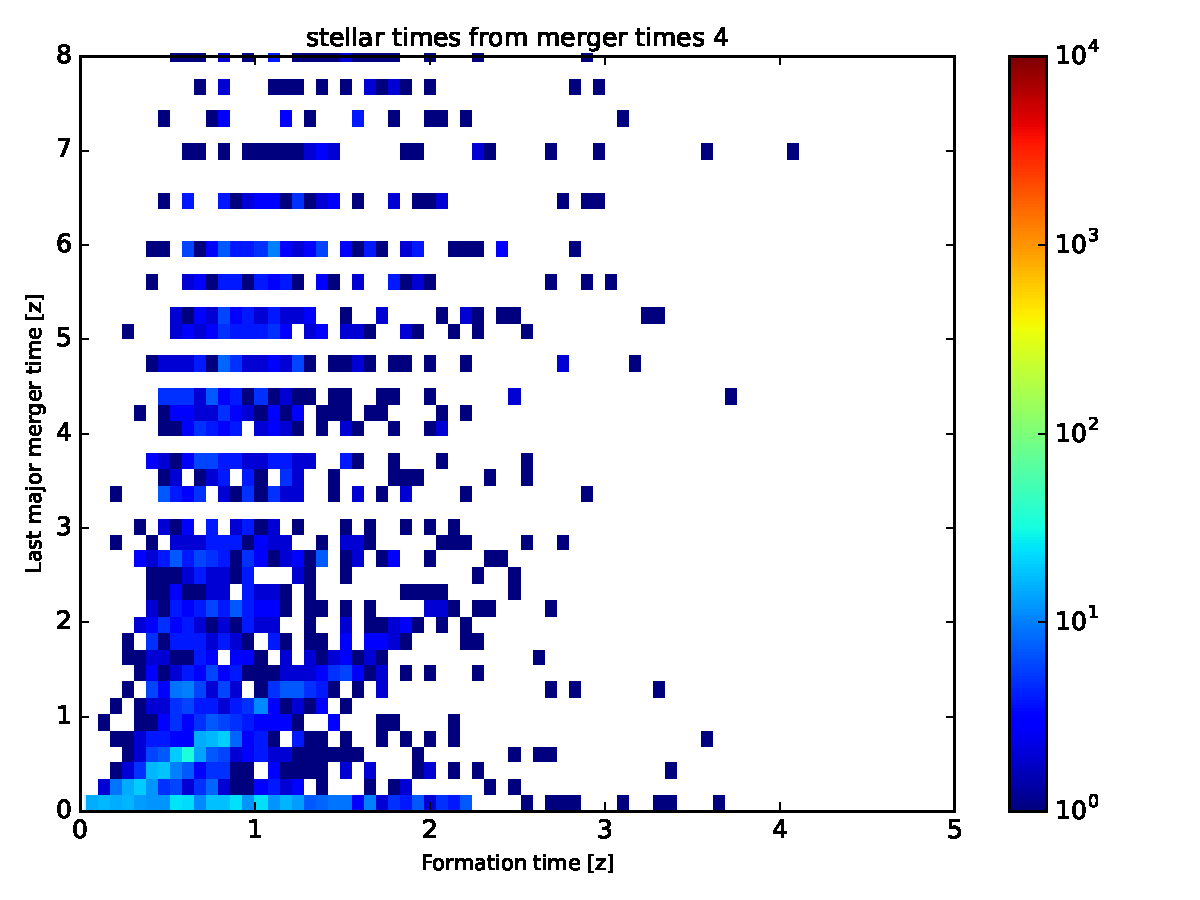
\includegraphics[scale=0.27]{avgProp/stellar_2DhistTimes_4.pdf}
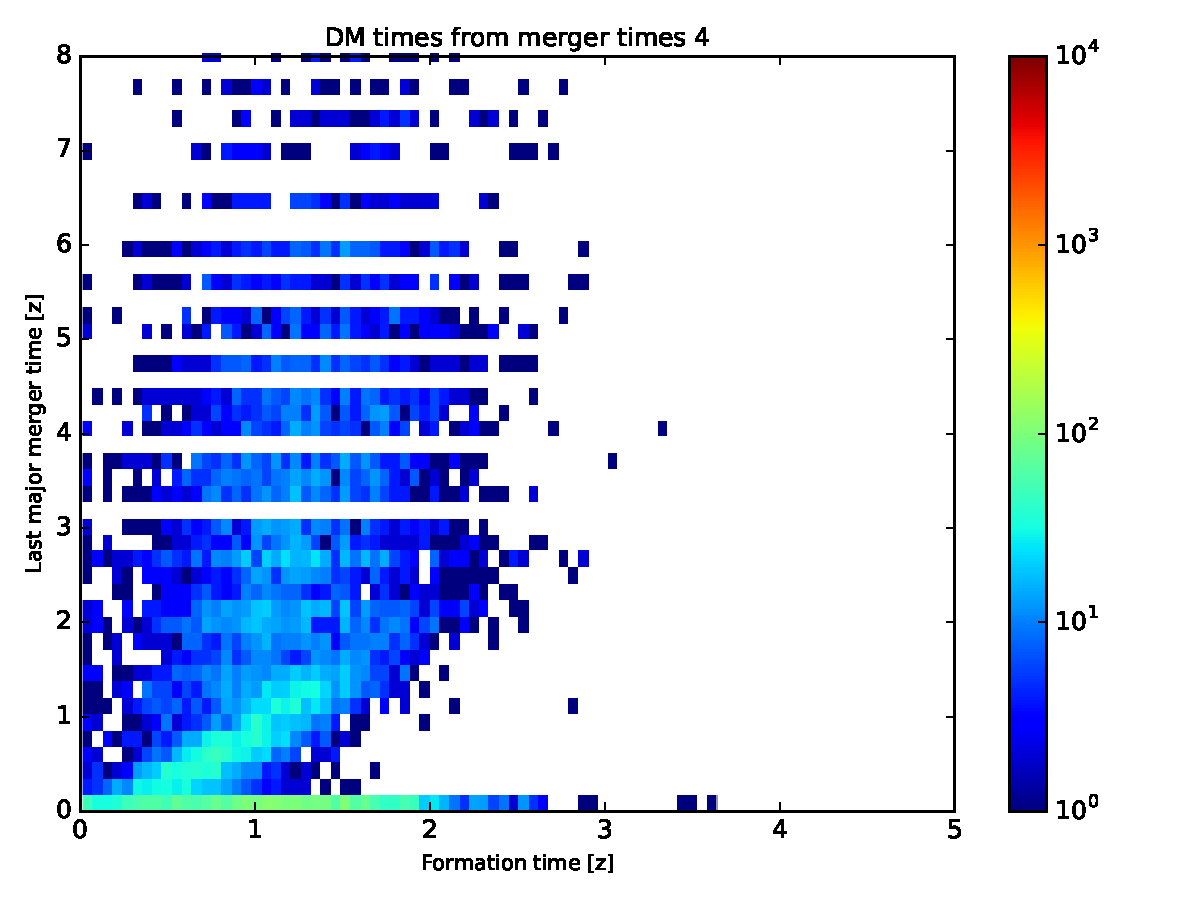
\includegraphics[scale=0.27]{avgProp/DM_2DhistTimes_4.pdf}
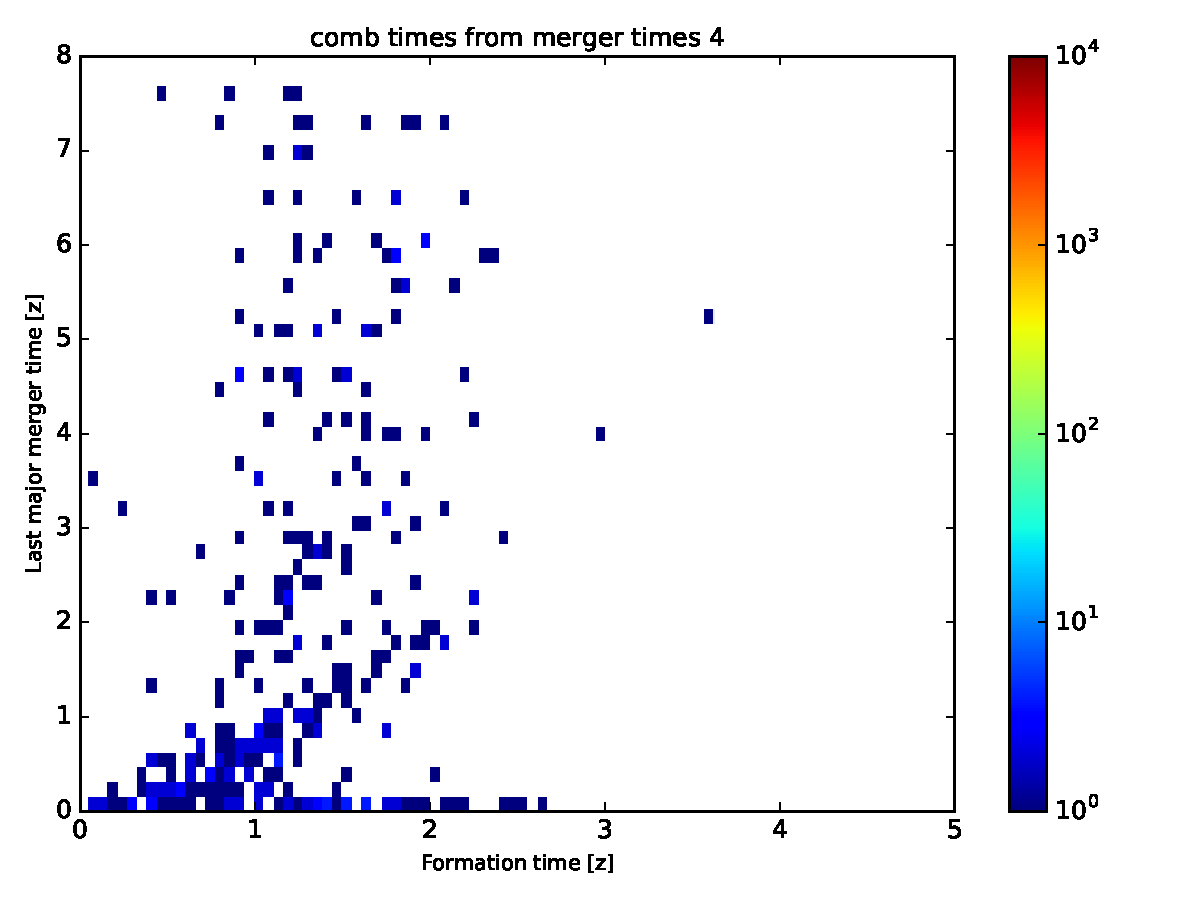
\includegraphics[scale=0.27]{avgProp/comb_2DhistTimes_4.pdf}
\caption{\label{fig:2d_times} 2D histograms of the last major merger times and formation times. From left to right: stellar mass, dark matter halo mass and broader observational values. Top row: distribution after applying the mass cut, bottom row: distribution after the velocity cut.}
\end{figure*}





\bibliographystyle{mnras}
\bibliography{references}



\end{document}
